\documentclass[12pt]{article}
\usepackage[margin=1in]{geometry}
\usepackage{amsmath,amsthm,amssymb,amsfonts}
\usepackage{graphicx}

\newcommand{\N}{\mathbb{N}}
\newcommand{\Z}{\mathbb{Z}}

\newenvironment{part}[2][Part]{\begin{trivlist}
\item[\hskip \labelsep {\bfseries #1}\hskip \labelsep {\bfseries #2.}]}{\end{trivlist}}
%If you want to title your bold things something different just make another thing exactly like this but replace "problem" with the name of the thing you want, like theorem or lemma or whatever

\newenvironment{writeup}[2][Write-Up]{\begin{trivlist}
\item[\hskip \labelsep {\bfseries #1}\hskip \labelsep {\bfseries #2.}]}{\end{trivlist}}

\graphicspath{ {./} }


\begin{document}

%\renewcommand{\qedsymbol}{\filledbox}
%Good resources for looking up how to do stuff:
%Binary operators: http://www.access2science.com/latex/Binary.html
%General help: http://en.wikibooks.org/wiki/LaTeX/Mathematics
%Or just google stuff

\title{AST 540: Lab 1}
\author{Jonas Powell}
\maketitle

\begin{part}{Measuring System Temperature Using Vane Calibration}
  Describe the calibration procedure and record the system temperature that you measure along with the time at which you measured it. Collect data from the other observing groups and make two plots:

  \bigskip
  (1) system temperature as a function of time throughout the day \\
  \indent(2) system temperature as a function of ambient temperature.


  \bigskip
  By how much does the system temperature fluctuate throughout the day? Does it seem to track the ambient temperature? How does the system temperature compare to the theoretical quantum limit on the receiver temperature for this system?
\end{part}

\begin{writeup}{1}

  To calibrate our system, we began by moving the dish to a point on the sky at the same altitude as our source and slewed in azimuth until we were off any other radio sources and pressed the "Cal" button on the SRT GUI to get a cold sky measurement. We then sent Hunter outside to put the "absorber-on-a-stick" in front of the antenna's receiver, pressed "Enter" as prompted by the GUI, and allowed it to complete it's measurement. In this process, we found power values of:

  \begin{align*}
    P_{\text{cold}} &= 179.3 \\
    P_{\text{hot}} &= 358.7
  \end{align*}

  We may then recall the Y-Factor calibration equations to solve for our receiver temperature.
  \begin{align*}
    y &= \frac{P_H}{P_C} = 2 \\
    T_{Rx} &= \frac{T_H - y T_C}{y - 1}
  \end{align*}

  where $T_H$ is the ambient temperature, $292$, amd $T_C$ is the cosmic microwave background, $2.7$. Then:

  \begin{align*}
    T_{Rx} &= \frac{292 - 2 \times 2.7}{2 - 1} \\
           &= 286.6
  \end{align*}


  Using other teams' data, we may make plots of system temperature. We find system temperature from the antenna temperature using the formula:

  \begin{center}
    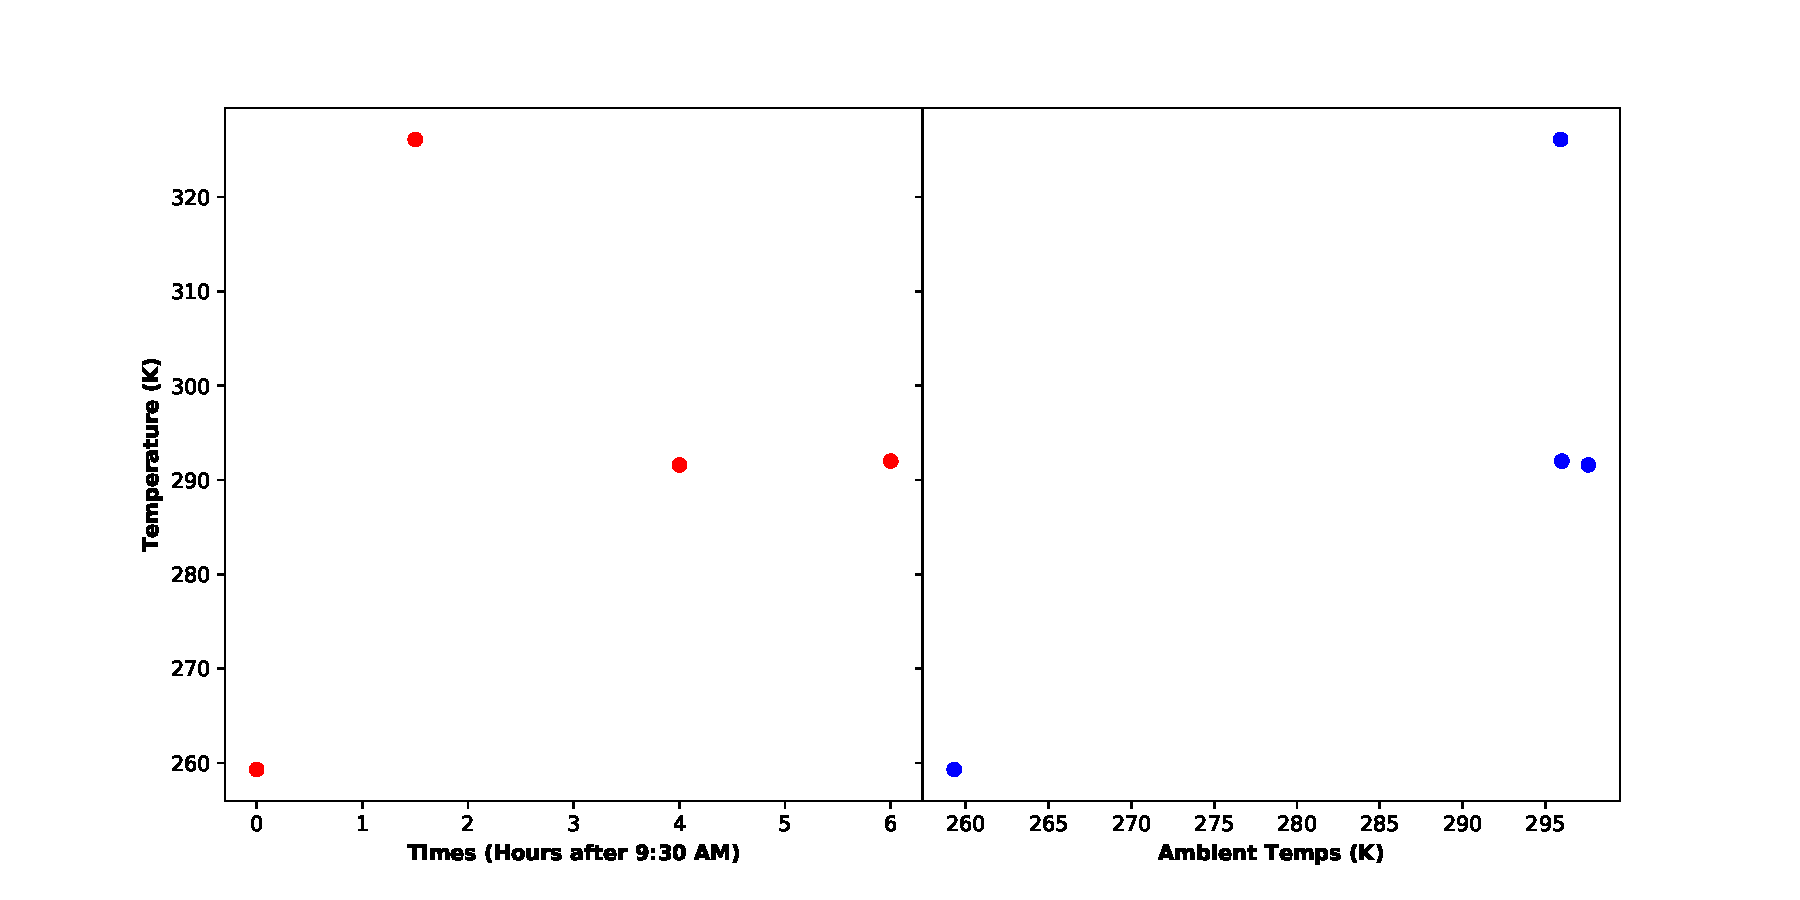
\includegraphics[scale=0.6]{sys_temps.pdf} \\
  \end{center}

It's hard to make any sense of these plots, since they only have four points and each has its own unrelated sets of uncertainties (each observing team's specific methods and errors).

\end{writeup}
\bigskip
\bigskip







\begin{part}{Measure Antenna Beamwidth using the Sun as a Signal Source}
  Generate two plots of antenna temperature as a function of degrees offset in (1) azimuth and (2) elevation. Measure the HPBW of the SRT antenna in both azimuth and elevation. Are they the same? Why or why not? (Hint: Since the Sun is unlikely to be near the horizon, you will need to be careful with the azimuth axis. Try to figure out the appropriate correction factor to apply, since circles of constant elevation are not great circles.)
  \bigskip

  How does your plot of the gain pattern of the antenna compare with what you would expect for a uniform circular aperture (2.4m in diameter, observing at a wavelength of 21cm)? Plot an Airy function over your data (you will need to add a vertical offset to account for the system temperature). How does the beamwidth you measured compare with the theoretical expectation? Do you see the sidelobe levels you expected to see?
  \bigskip

  One reason your data will not match the theoretical expectation is that the aperture is undergoing nonuniform illumination (another reason is that the feed may be slightly out of focus). The tapered illumination caused by the beam pattern of the feed can be well approximated by the following function:
  \begin{align*}
    \epsilon(\rho) = [1 – (2\rho/D)^2]^{\gamma}
  \end{align*}
  Which results in a gain pattern
  \begin{align*}
    G(\theta) = [2\gamma+1 (\gamma+1)!]^2 \,\, [4\pi A_g / \lambda^2] \,\, \left(\frac{J_{\gamma+1}(\pi D \theta/\lambda)}{(\pi D \theta/\lambda)^2} \right) ^2
  \end{align*}
  \bigskip

  For most real-life feeds, $\gamma \approx 1$. Try plotting the gain pattern for $\gamma = 1$, and see if it provides any improvement over the Airy pattern expected for the uniform illumination condition.
\end{part}

\begin{writeup}{2}
  We may convert our power measurements to antenna temperature by recalling
  \begin{align*}
    P &= k_B G B T \\
    P &= cT, \,\,\,\,\,\, c = k_B G B
  \end{align*}

  Since we are just looking for a conversion factor, we don't need to solve this equation for $c$ with actual values, but can instead solve it for the hot and cold temperature observations and just use the resulting value as an offset. Using our observed values of:
  \begin{align*}
    T_H &= 1 \\
    T_C &= 1 \\
  \end{align*}
  blah
  \begin{align*}
    y &= \frac{P_H}{P_C} \\
      &= \frac{T_H + T_{rx}}{T_C + T_{Rx}} \\
    \rightarrow T_{Rx} &= T_H - \frac{y T_C}{y - 1} \\
  \end{align*}

  With our value for $T_{Rx}$ in hand we can now solve for our constant, $c$:

  \begin{align*}
    P_H &= c_H \left(T_H + T_{Rx} \right), \,\,\,  P_C = c_C \left(T_C + T_{Rx} \right) \\
    c_H &= \frac{P_H}{T_H + T_{Rx}}, \,\,\, c_C = \frac{P_C}{T_C + T_{Rx}} \\
  \end{align*}

  Finally, we plug in values and hope that our resulting values for $c$ are the same:
  \begin{align*}
    P_H &= 358.7, \,\, P_C = 179.4 \\
    \rightarrow y &= 2 \\
    T_H &= 297.59, \,\, T_C = 2.7 \\
    \rightarrow T_{Rx} &= 297.59 - \frac{2 T_C}{2-1} = 292.19 \\
    c_H &= \frac{358.7}{297.59 + 292.19}, \,\, c_C = \frac{179.4}{2.7 + 292.19} \\
        &= 0.6 \\
  \end{align*}

  Hurrah! As expected, the receiver's bias is constant. Using that constant, we may now convert all our power measurements to antenna temperatures by dividing them by $c$ and plot them:

  \bigskip
  \begin{center}
    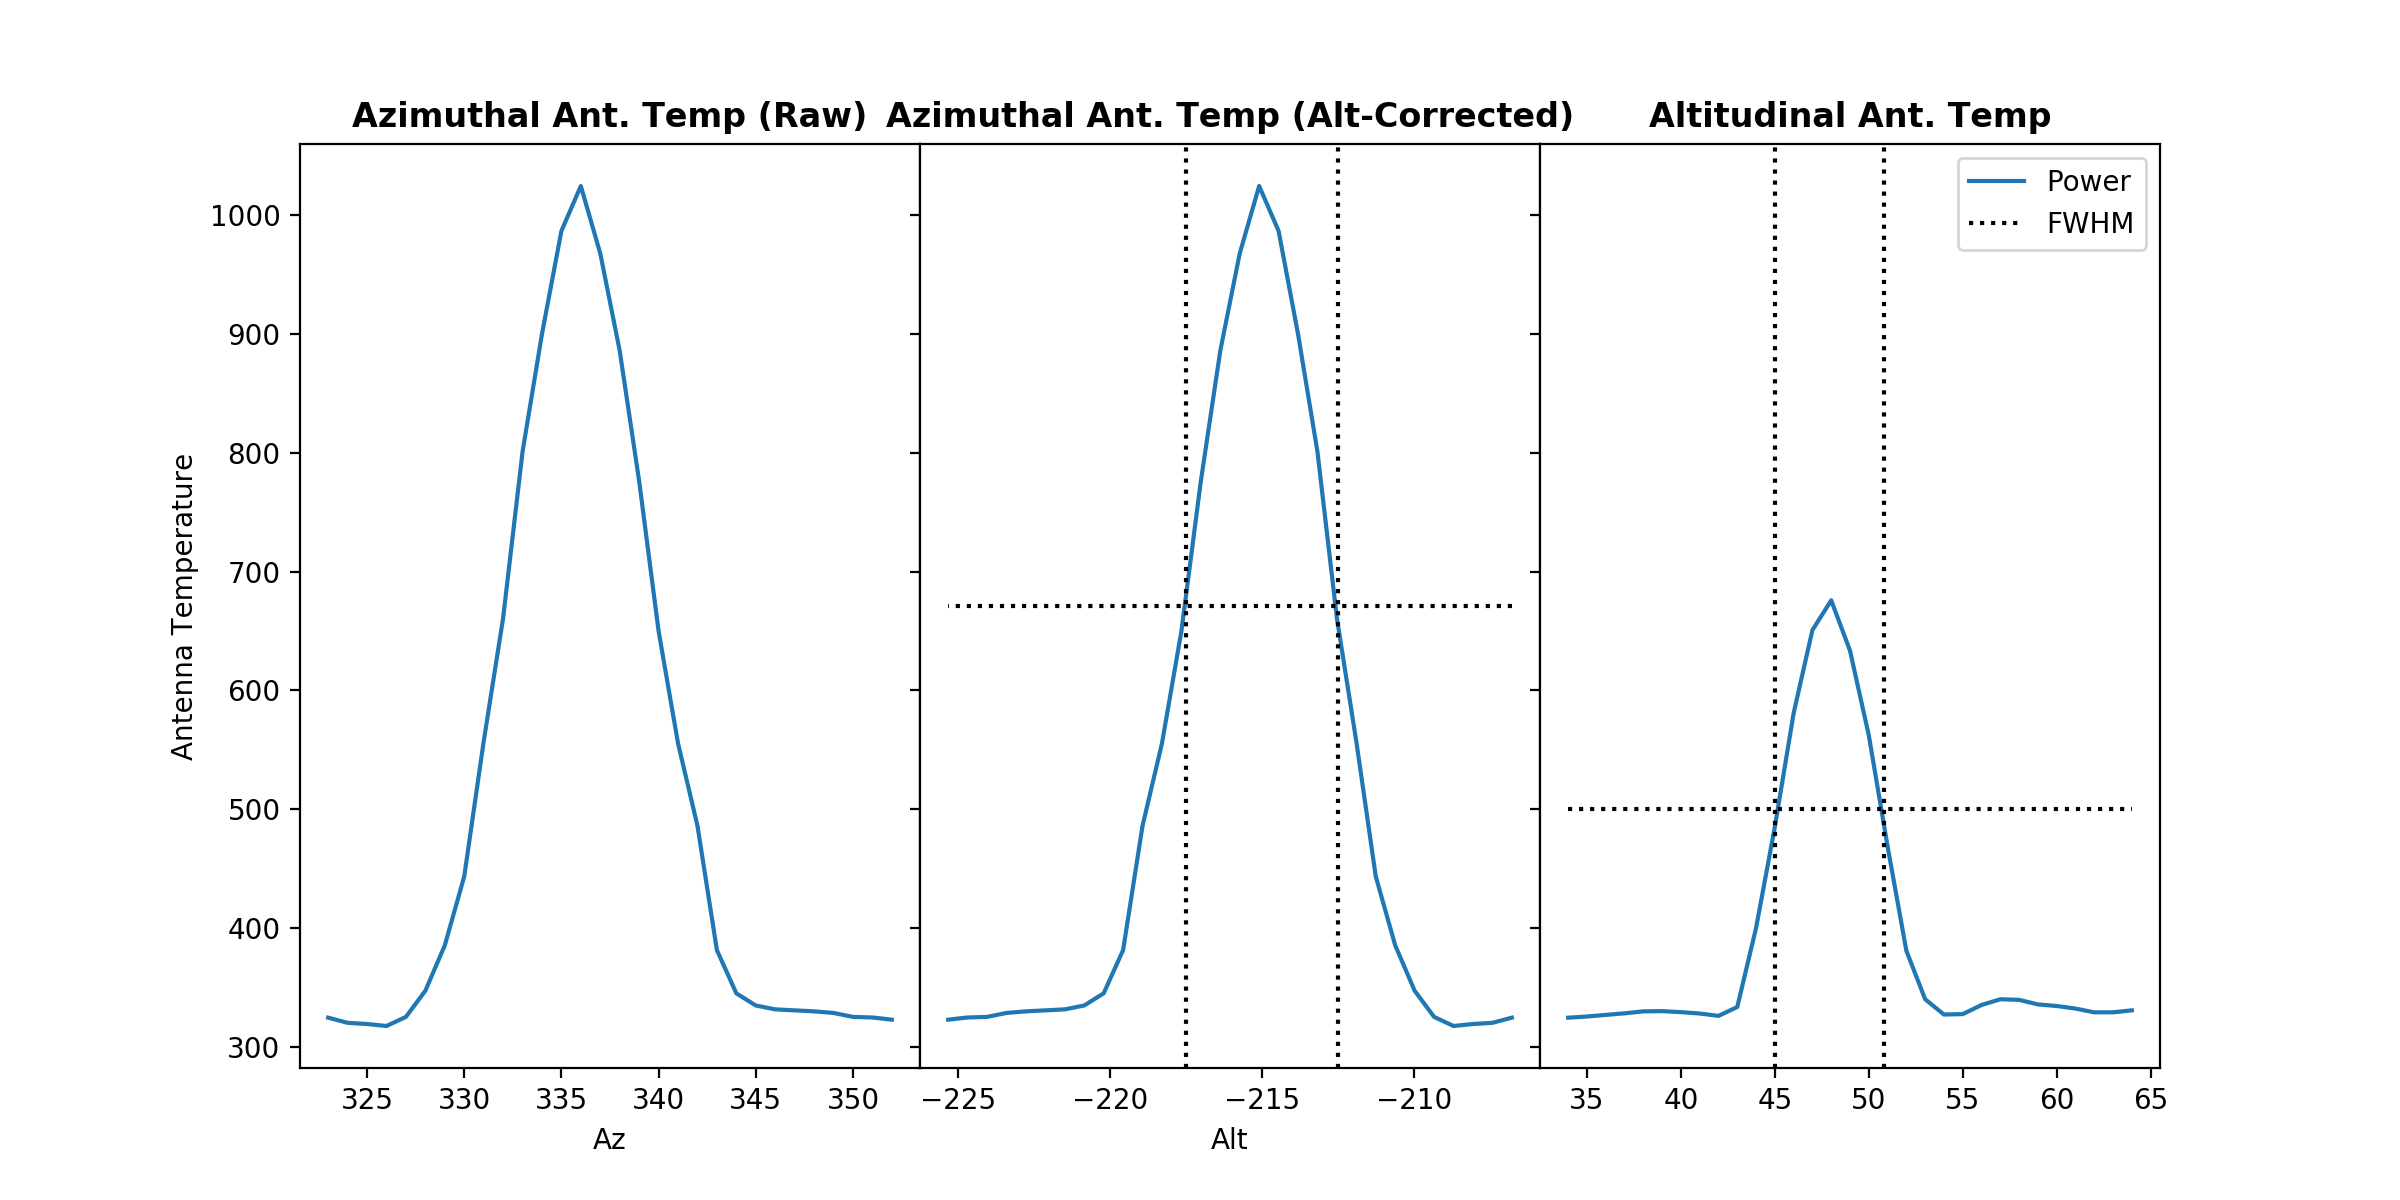
\includegraphics[scale=0.5]{part1_1} \\
    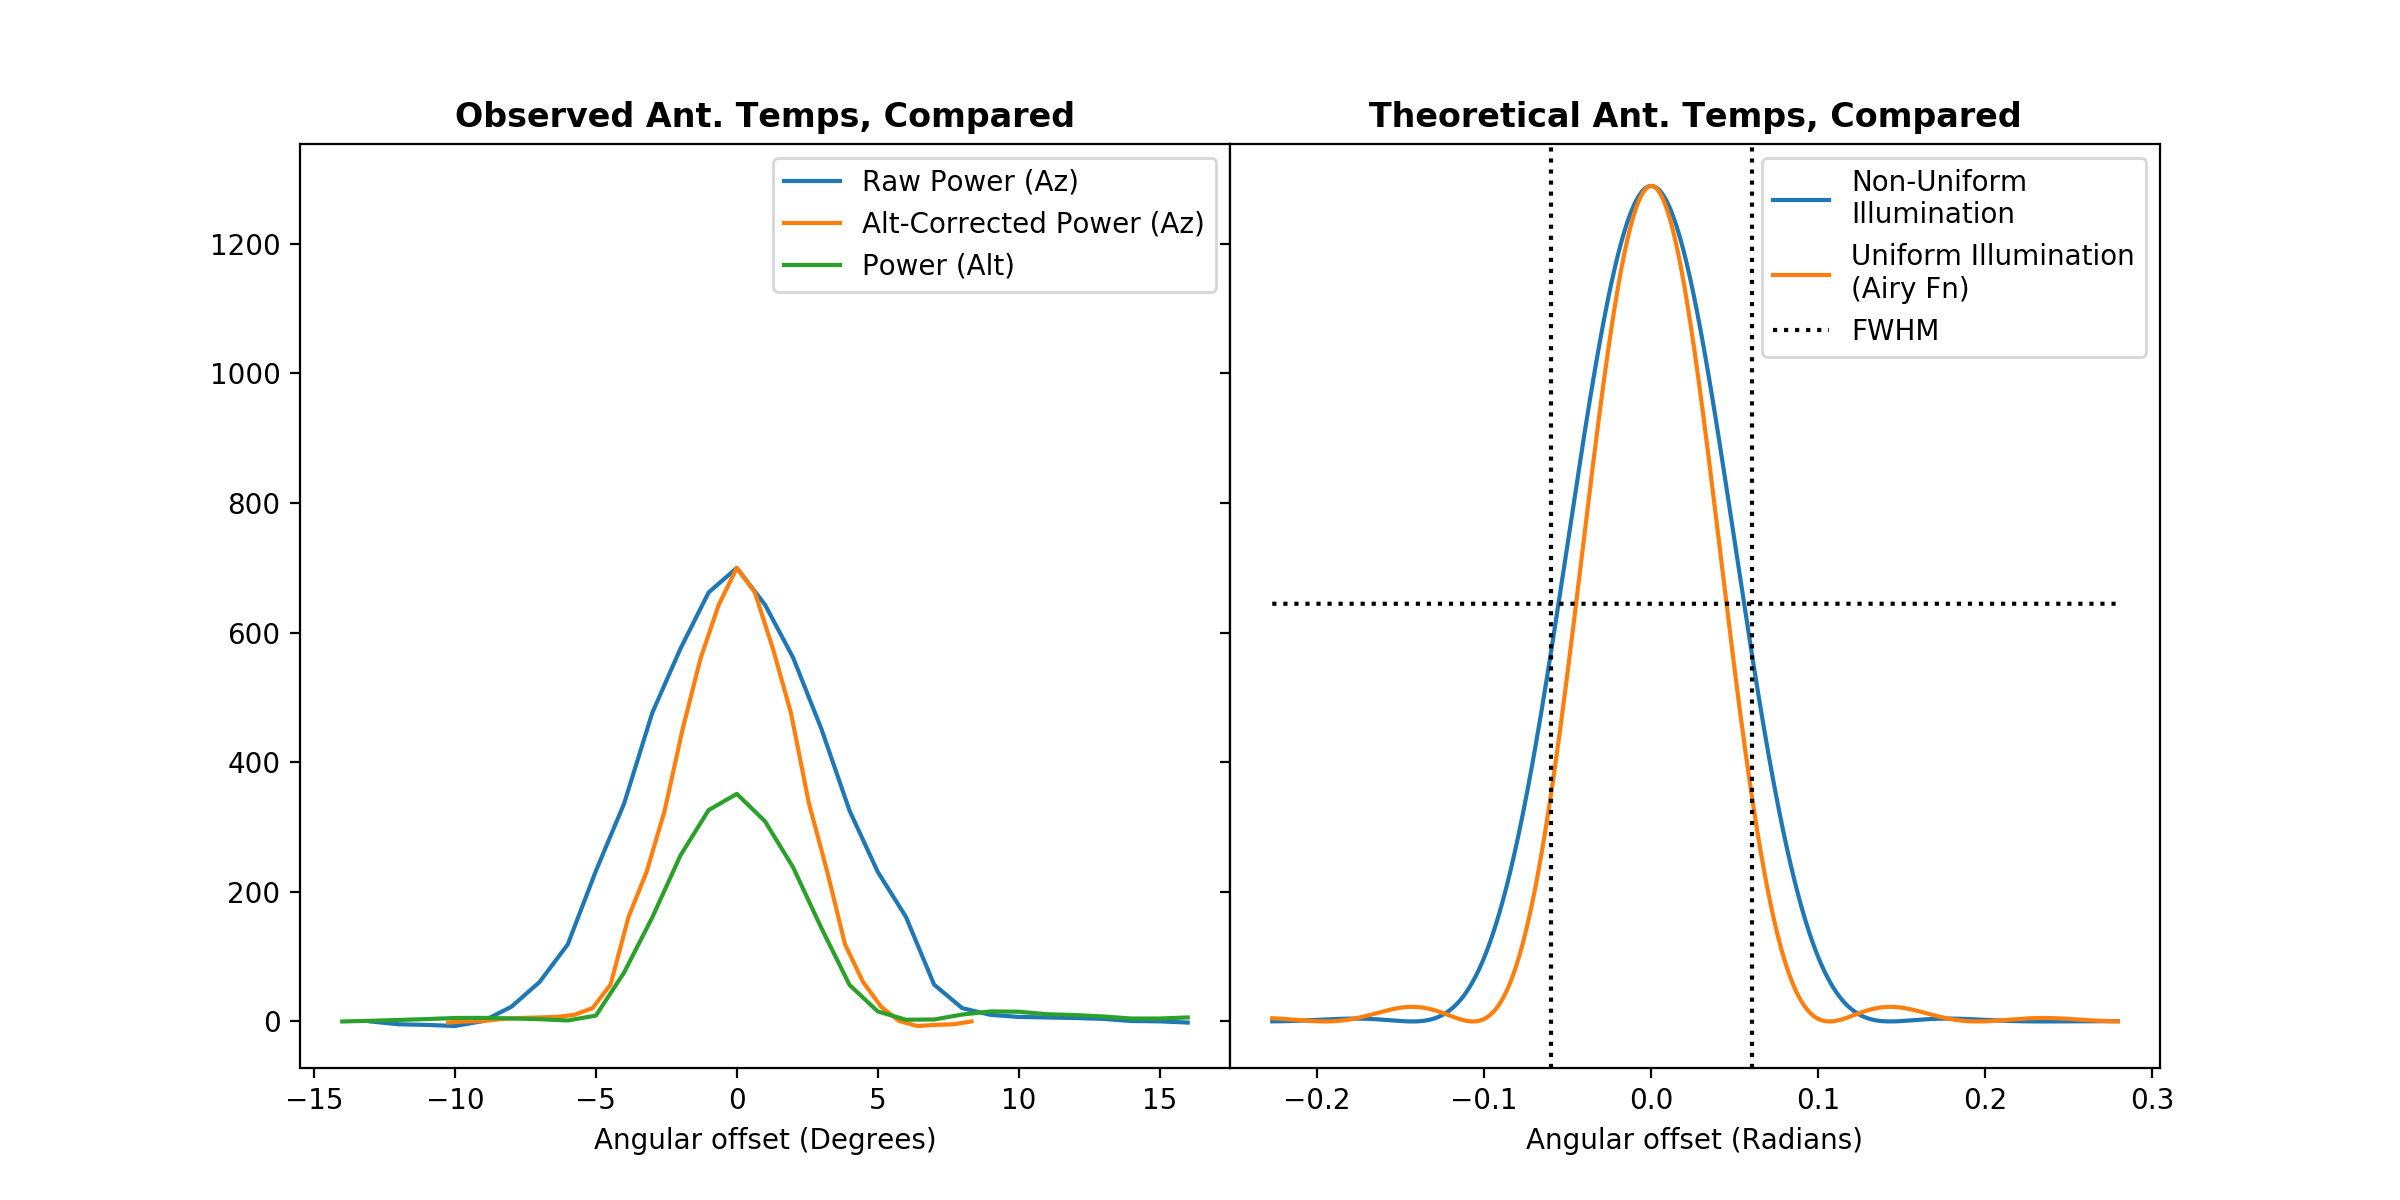
\includegraphics[scale=0.5]{part1_2} \\
  \end{center}

In the first two panels of the upper plot, we plot the power we recorded (converted to temperature): on the left is the "raw" data, while in the middle, the azimuth values have been multiplied by a factor of $\cos 48^o$ to compensate for the fact that azimuthal circles at non-equatorial altitudes are not great circles. In the left hand plot on the bottom, we see that this correction recovers the beam's angular symmetry (although the amplitudes of the altitudinal/azimuthal power measurement's are different). Finally, plotted in the bottom right we see the gain patterns predicted by the gain patterns of a uniformly and non-uniformly illuminated aperture.

Using the dotted lines as visual guides to finding our FWHM values, we find that:

\begin{align*}
  \text{FWHM}_{\text{Az}} &= 5^o \\
  \text{FWHM}M_{\text{Alt}} &= 5.8^o \\
  \text{FWHM}_{\text{Theoretical}} &= 0.14 \text{ radians} = 8^o \\
\end{align*}

Therefore, we see that although the amplitudes of our observations are pretty far below those predicted by the theoretical gain functions (which don't vary signiicantly between uniform and non-uniform illumination patterns), the FWHMs are still in similar ballparks and our observed beam is pretty darn close to symmetric.
\bigskip
\bigskip





\begin{part}{Measure Aperture Efficiency}
  Calculate the aperture efficiency of the SRT, making sure to properly account for the system temperature. Look up the angular diameter of the Sun (cite your source) and use it along with your previous measurements of antenna temperature and aperture efficiency to estimate the flux density of the Sun at a wavelength of 21 cm. Collect your classmates’ measurements and plot the Solar flux as a function of time throughout the day (we might see a flare!).
  \bigskip
  \bigskip

\end{part}

\begin{writeup}{3}

  We begin by finding the Sun's diameter from Wolfram Alpha:
  \begin{align*}
    R_{\odot} &= 1.391 \times 10^{9} \text{ meters}
  \end{align*}

We may use the equations given to formulate an equation for the aperture efficiency of the SRT.

\begin{align*}
  \eta &= \frac{A_e}{A_G} \\
       &= \frac {2kT_A}{FA_g} \\
\end{align*}


We know that:
\begin{align*}
  F &= 2000 \text{ Jy} \\
  A &= 4.52 \text{ meters}^2
\end{align*}

This leaves us with the task of solving for $T_A$. Since the loop that was explained in the assignment didn't make sense to me, I decided to approximate it by simply subtracting the off-source power measurements from the on-source ones and taking the average value of this difference (and removing a couple bad measurements). Although this loses some of the specific directional averaging given by the loop in the assignment, I think that it is somewhat close to what is being asked. This process gave me a value of $P_{ave} = 10.75$. To convert this to a temperature, we use our constant $c = 0.6$ to scale it and get the units right, leaving us with:
$T_A &= 17.9$ K.

Plugging all these values into Wolfram, we in an efficiency value of $\eta = 5.34$. This is obviously a ridiculous result, since the efficiency should be $\le 1$. The problem is coming from the value for $T_A$, which came from my interpretation of the given loop and potentially bad data. We were thinking that perhaps synchrotron radiation might be responsible for at least a little bit of this over-observation (since the efficiency is only relative to the flux of Cas A), but it seems extremely unlikely to me that there is enough of that radiation to justify that extreme abundance.


\bigskip
\bigskip


The link is broken and so we are unable to find solar flux values.

\end{writeup}


\end{document}
